\chapter{Linear Regression Results}
\label{chap:regression-linear}

\section{Descriptive Overview of the Scenarios}
The linear regression experiments covered 972 scenarios for continuous predictors and 972 for binary predictors (before cross-referencing with all error and correlation levels). The success rate for model fitting was 100\% across all linear scenarios, as the continuous nature of the outcome avoids the convergence issues typical of discrete models.

\begin{table}[H]
    \centering
    \caption[Summary of experimental factors for Linear Regression]{Summary of experimental factors for Linear Regression simulations.}
    \label{tab:linear-factors}
    \begin{tabular}{@{}ll@{}}
        \toprule
        \textbf{Factor} & \textbf{Evaluated Levels} \\ \midrule
        Sample Size ($N$) & 100, 500, 1000 \\
        Predictors ($p$) & 2, 5, 10 \\
        Correlation ($\rho$) & 0.0, 0.3, 0.6 \\
        Error Variance ($\sigma^2$) & 0.5, 1.0, 2.0 \\
        Variable Types & Continuous, Binary \\
        Synthesis Methods & CART, Parametric (Normal) \\ \bottomrule
    \end{tabular}
    \source{Compiled by the author}
\end{table}

\section{Univariate Analysis of Inferential Utility}
This section examines how individual design factors influence the Confidence Interval Overlap (CIO), averaging across all other dimensions.
Figure~\ref{fig:linear-cio-univariate} summarizes the univariate CIO trends for the linear-regression scenarios.

\begin{figure}[H]
    \centering
    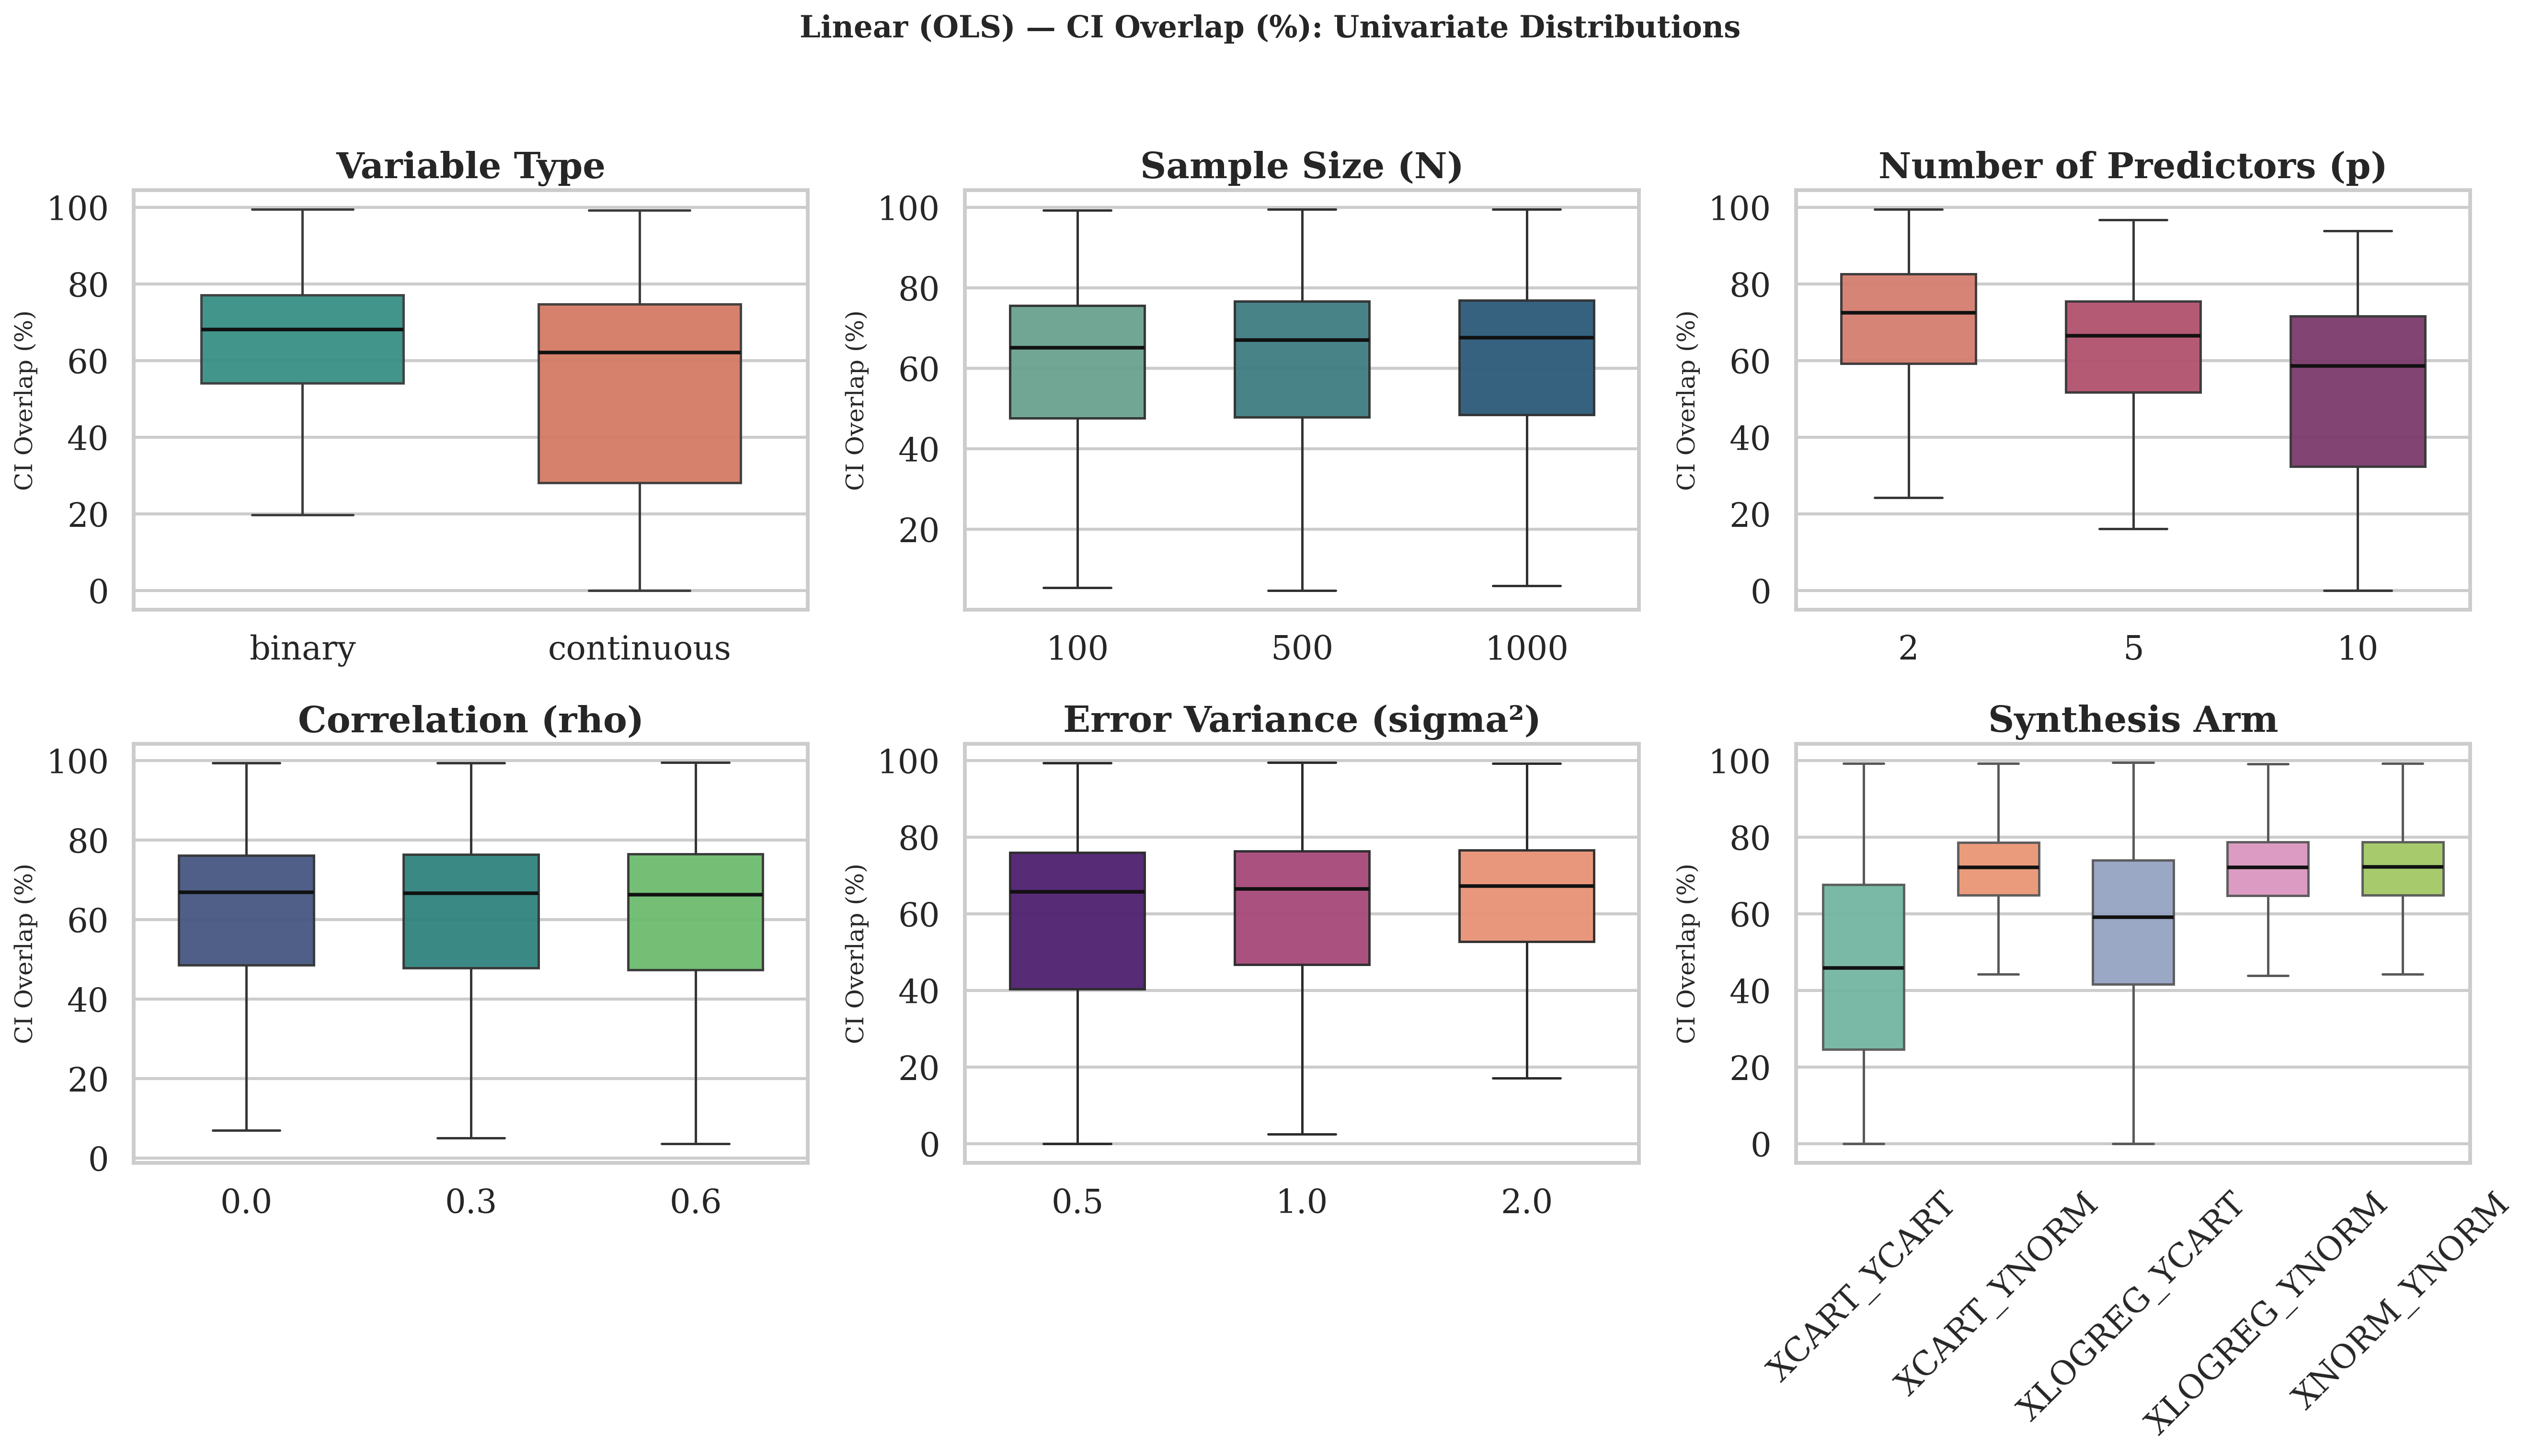
\includegraphics[width=0.8\textwidth]{figures/parts/03_Regression/03_Linear_Results/linear_cio_univariate.png}
    \caption[Univariate analysis of CIO for Linear Regression]{Univariate analysis of CIO for Linear Regression across Sample Size (N), Number of Predictors (p), and Correlation (rho).}
    \label{fig:linear-cio-univariate}
    \source{Compiled by the author}
\end{figure}

\subsection{Analysis by Sample Size}
As shown in Figure~\ref{fig:linear-cio-univariate}, sample size ($N$) has a stabilizing effect on CIO. From a statistical perspective, the variance of the Ordinary Least Squares (OLS) estimator $\hat{\beta}$ is inversely proportional to the sample size:
\begin{equation}
    \text{Var}(\hat{\beta}) = \sigma^2 (\mathbf{X}^T \mathbf{X})^{-1} \propto \frac{1}{N}
\end{equation}
While the average overlap remains high (> 0.8), larger sample sizes reduce the variance of the estimates, leading to more consistent synthetic reproduction of the original results. The asymptotic properties of maximum likelihood estimation ensure that as $N \to \infty$, the empirical distribution generated by the synthesis model closely matches the true underlying distribution, thereby stabilizing the synthetic Confidence Intervals.

\subsection{Analysis by Number of Predictors}
The dimensionality ($p$) shows a slight downward trend in utility. As the number of predictors increases from 2 to 10, the complexity of the conditional generation sequence grows. In sequential synthesis, each variable $X_j$ is modeled conditional on all preceding variables $X_1, \dots, X_{j-1}$. By the chain rule of probability:
\begin{equation}
    P(X_1, \dots, X_p) = P(X_1) \prod_{j=2}^{p} P(X_j \mid X_1, \dots, X_{j-1})
\end{equation}
Errors in the estimation of early conditional models propagate multiplicatively through the sequence. Consequently, high-dimensional spaces introduce compounding structural artifacts that lead to a marginal but observable decrease in the average CIO.

\subsection{Analysis by Variable Type}
Continuous predictors generally yield higher CIO than binary predictors in linear models. This phenomenon occurs because the parametric ``Normal'' generator accurately characterizes the true multivariate Gaussian distribution $\mathcal{N}(\mu, \Sigma)$ from which continuous variables were drawn. Conversely, synthesizing binary predictors requires an intermediate probability estimation step (e.g., logistic thresholding):
\begin{equation}
    \hat{P}(X_j=1 \mid \mathbf{X}_{<j}) = \frac{1}{1 + \exp(-\mathbf{X}_{<j} \gamma)}
\end{equation}
This discretization step inherently introduces stochastic noise and mapping errors, perturbing the linear relationships required by the final OLS model.

\subsection{Analysis by Correlation and Error Variability}
High correlation ($\rho = 0.6$) between predictors consistently degrades the CIO. In standard linear regression, the variance of the estimated coefficient $\hat{\beta}_j$ is influenced by the Variance Inflation Factor (VIF):
\begin{equation}
    \text{Var}(\hat{\beta}_j) = \frac{\sigma^2}{(N-1)\text{Var}(X_j)} \cdot \frac{1}{1 - R_j^2}
\end{equation}
where $R_j^2$ is the coefficient of determination when regressing $X_j$ on the other $p-1$ predictors. The ``multicollinearity effect'' means that as $\rho$ increases, $1 - R_j^2$ approaches zero, drastically inflating the variance. In synthetic generation, preserving highly collinear structures without introducing structural noise is difficult. In this setting, tree-based sequential generators can have more trouble isolating the unique marginal contribution of each highly correlated variable, which can lead to shifted point estimates and expanded synthetic confidence intervals.

\section{Multivariate Comparison by Generator}
Figure~\ref{fig:linear-cio-method} compares CIO across the two main synthesis arms for linear regression.

\begin{figure}[H]
    \centering
    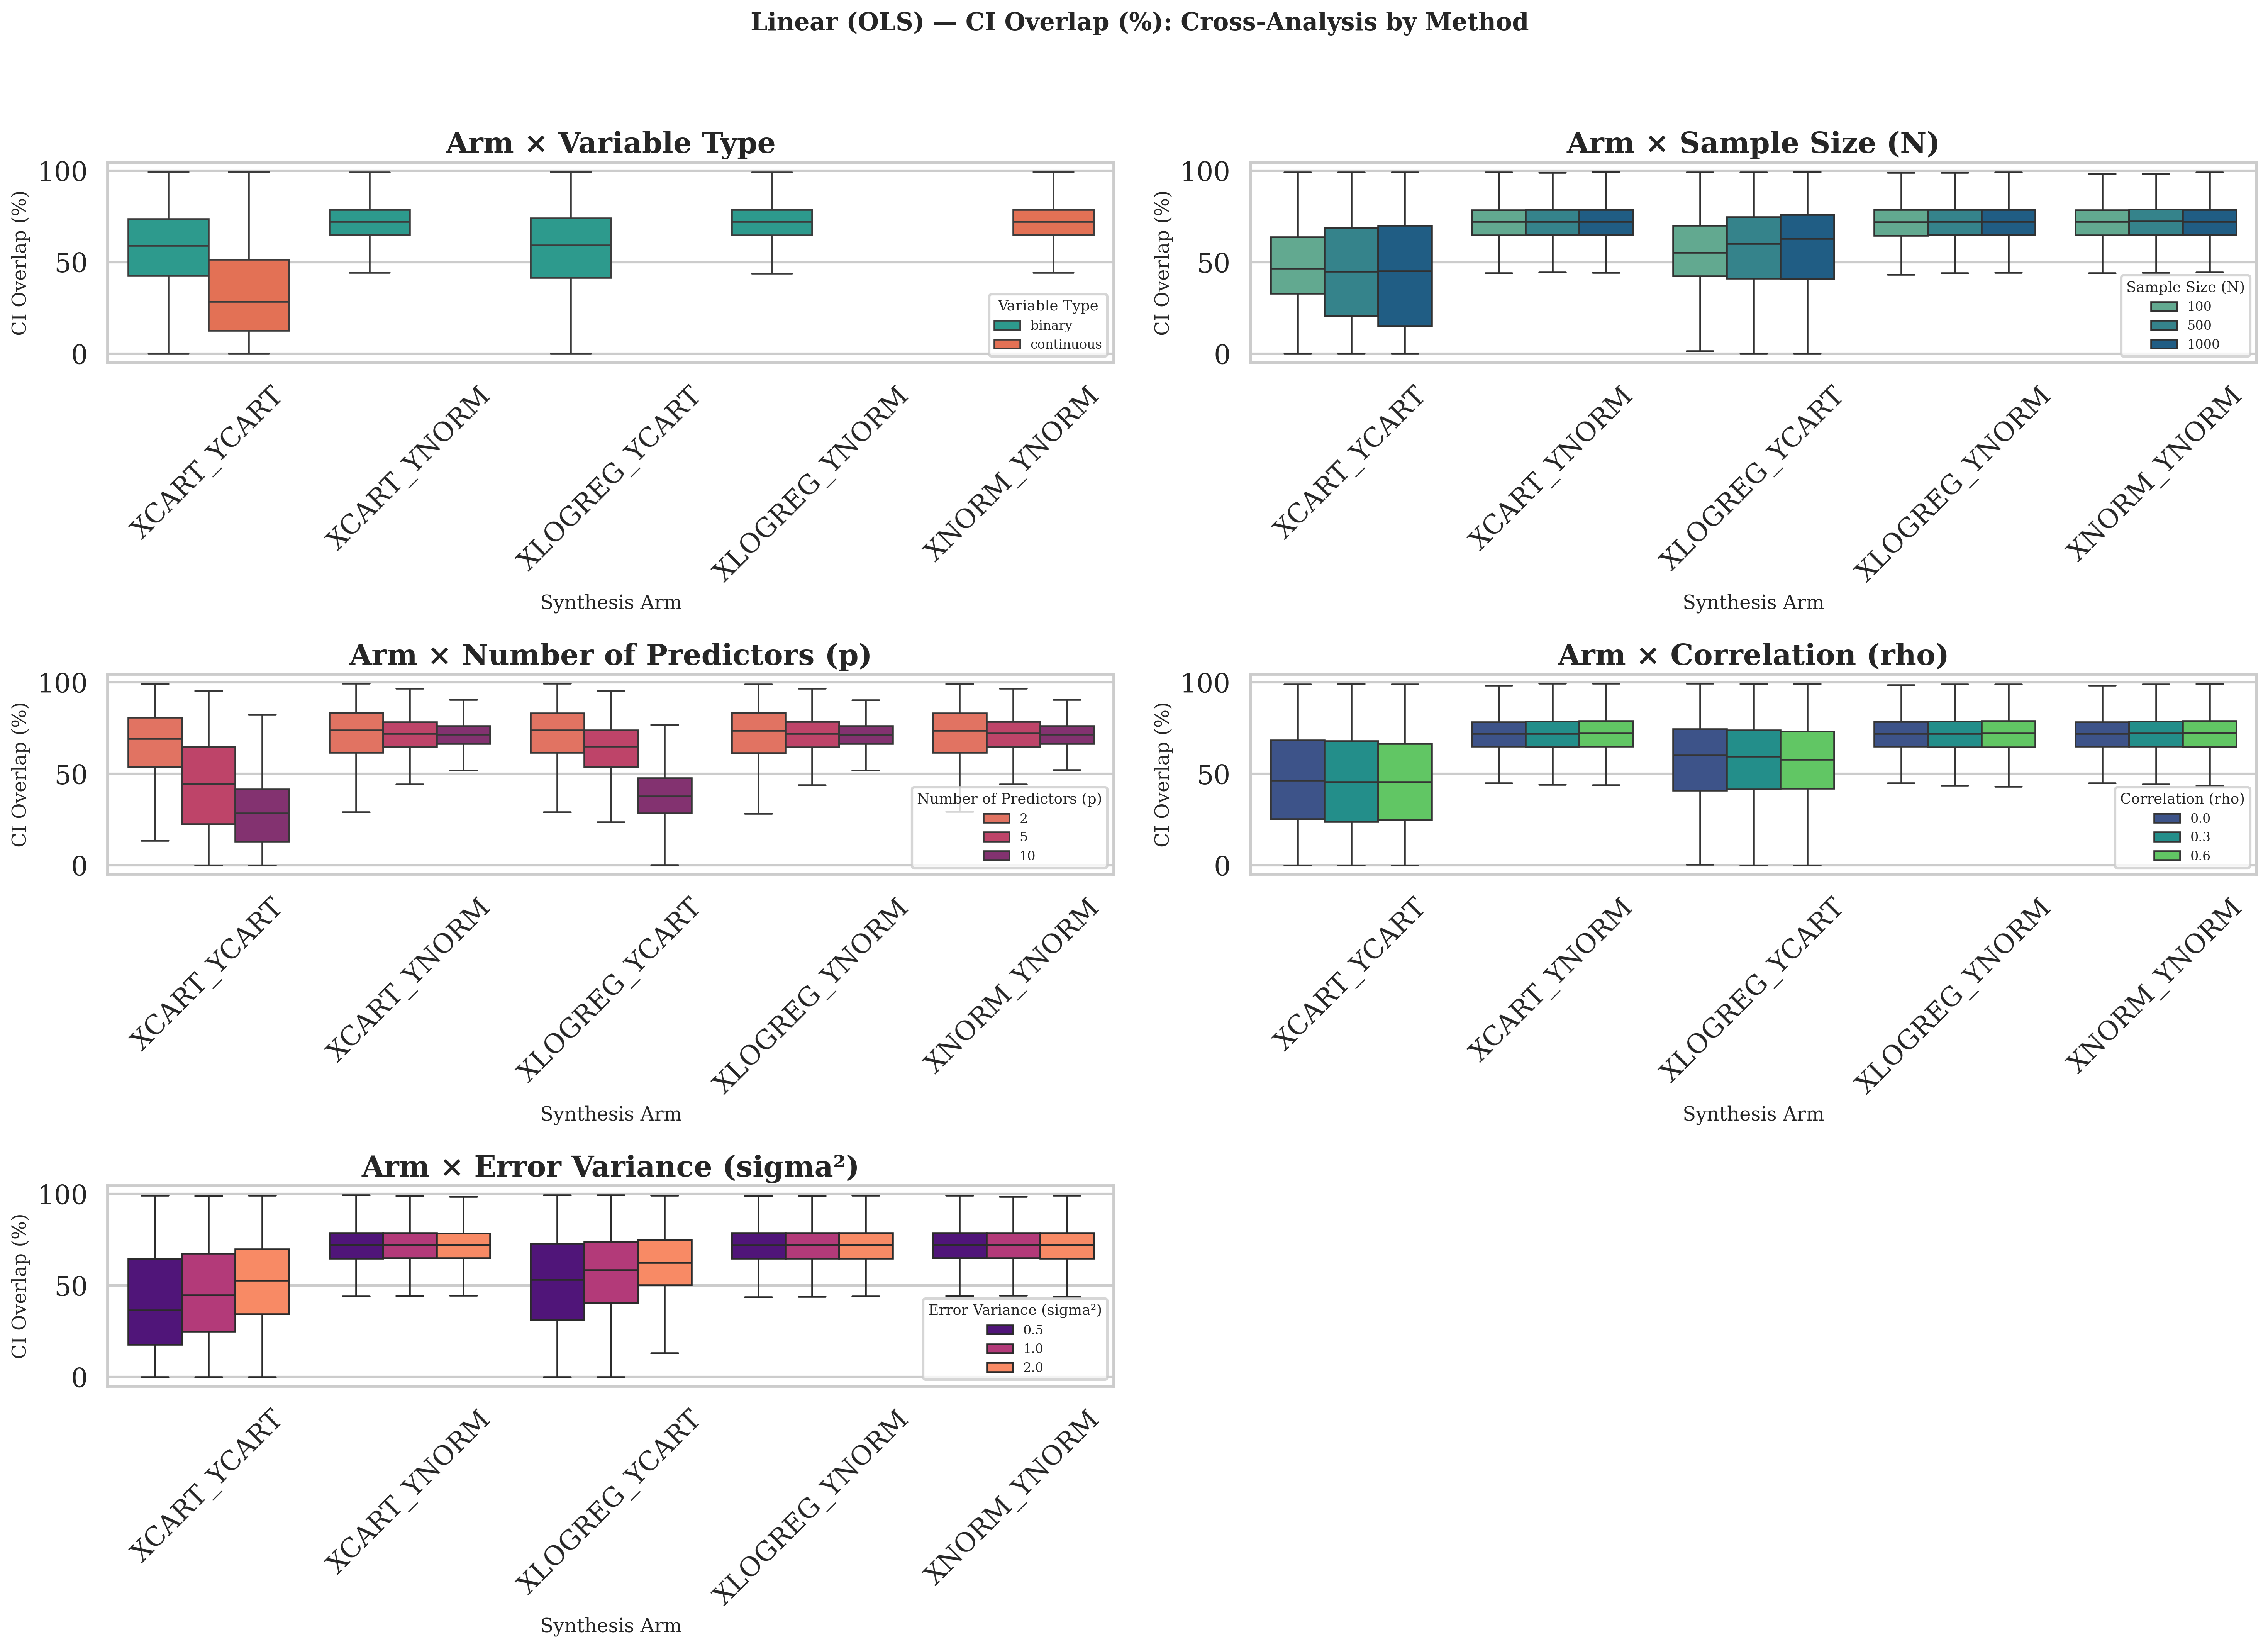
\includegraphics[width=0.8\textwidth]{figures/parts/03_Regression/03_Linear_Results/linear_cio_by_method.png}
    \caption[Comparison of CIO for Linear Regression]{Comparison of CIO across synthesis methods (CART vs. Parametric) for Linear Regression.}
    \label{fig:linear-cio-method}
    \source{Compiled by the author}
\end{figure}

Figure~\ref{fig:linear-cio-method} indicates that the \textbf{Parametric (Normal)} generator tends to achieve slightly higher CIO than CART in the linear-regression scenarios, although both methods remain usable across much of the design space. This pattern is consistent with the fact that the original data were generated under a linear, normal-error framework that is well aligned with the parametric synthesis assumptions.

\section{Interpretation of the Main Patterns}
Figure~\ref{fig:linear-heatmap} reports the Spearman correlation heatmap linking the main design factors to CIO.

\begin{figure}[H]
    \centering
    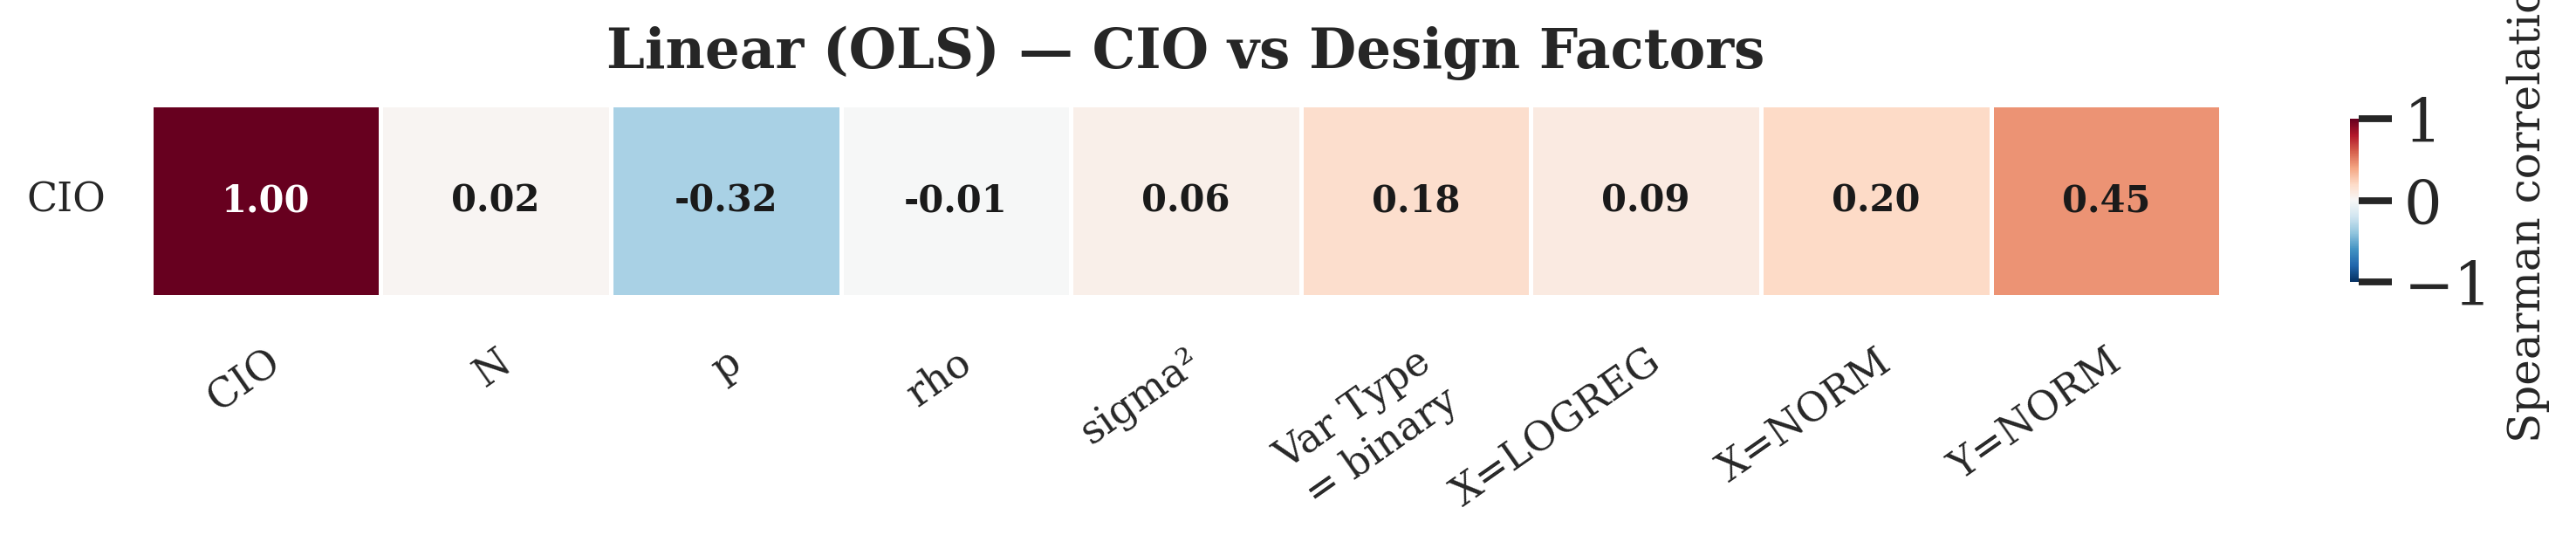
\includegraphics[width=0.9\textwidth]{figures/parts/03_Regression/03_Linear_Results/linear_cio_vs_design_correlation_spearman.png}
    \caption[CIO correlation heatmap for Linear Regression]{Spearman correlation heatmap between design factors and CIO for Linear Regression.}
    \label{fig:linear-heatmap}
    \source{Compiled by the author}
\end{figure}

The heatmap in Figure~\ref{fig:linear-heatmap} confirms the univariate findings: the number of predictors ($p$) and correlation ($\rho$) are the strongest negative drivers of CIO. Interestingly, the interaction between $p$ and $\rho$ suggests that synthetic data is most vulnerable when the model is both high-dimensional and highly correlated.

\section{Supporting Evidence from Bias and CI Width}

The CIO metric provides a holistic view of inferential utility, but it can be mathematically unpacked into two primary components: the displacement of the point estimate ($\Delta \hat{\beta}$) and the distortion of the standard error. We define the Bias Ratio as $B_R = |\hat{\beta}^{(S)} - \hat{\beta}^{(R)}| / \text{SE}(\hat{\beta}^{(R)})$ and the CI Width Ratio as $W_R = \text{Width}^{(S)} / \text{Width}^{(R)}$.

\subsection{Analysis of the Bias Ratio}
Figure~\ref{fig:linear-bias-ratio} shows the distribution of the Bias Ratio across synthesis methods for linear regression.

\begin{figure}[H]
    \centering
    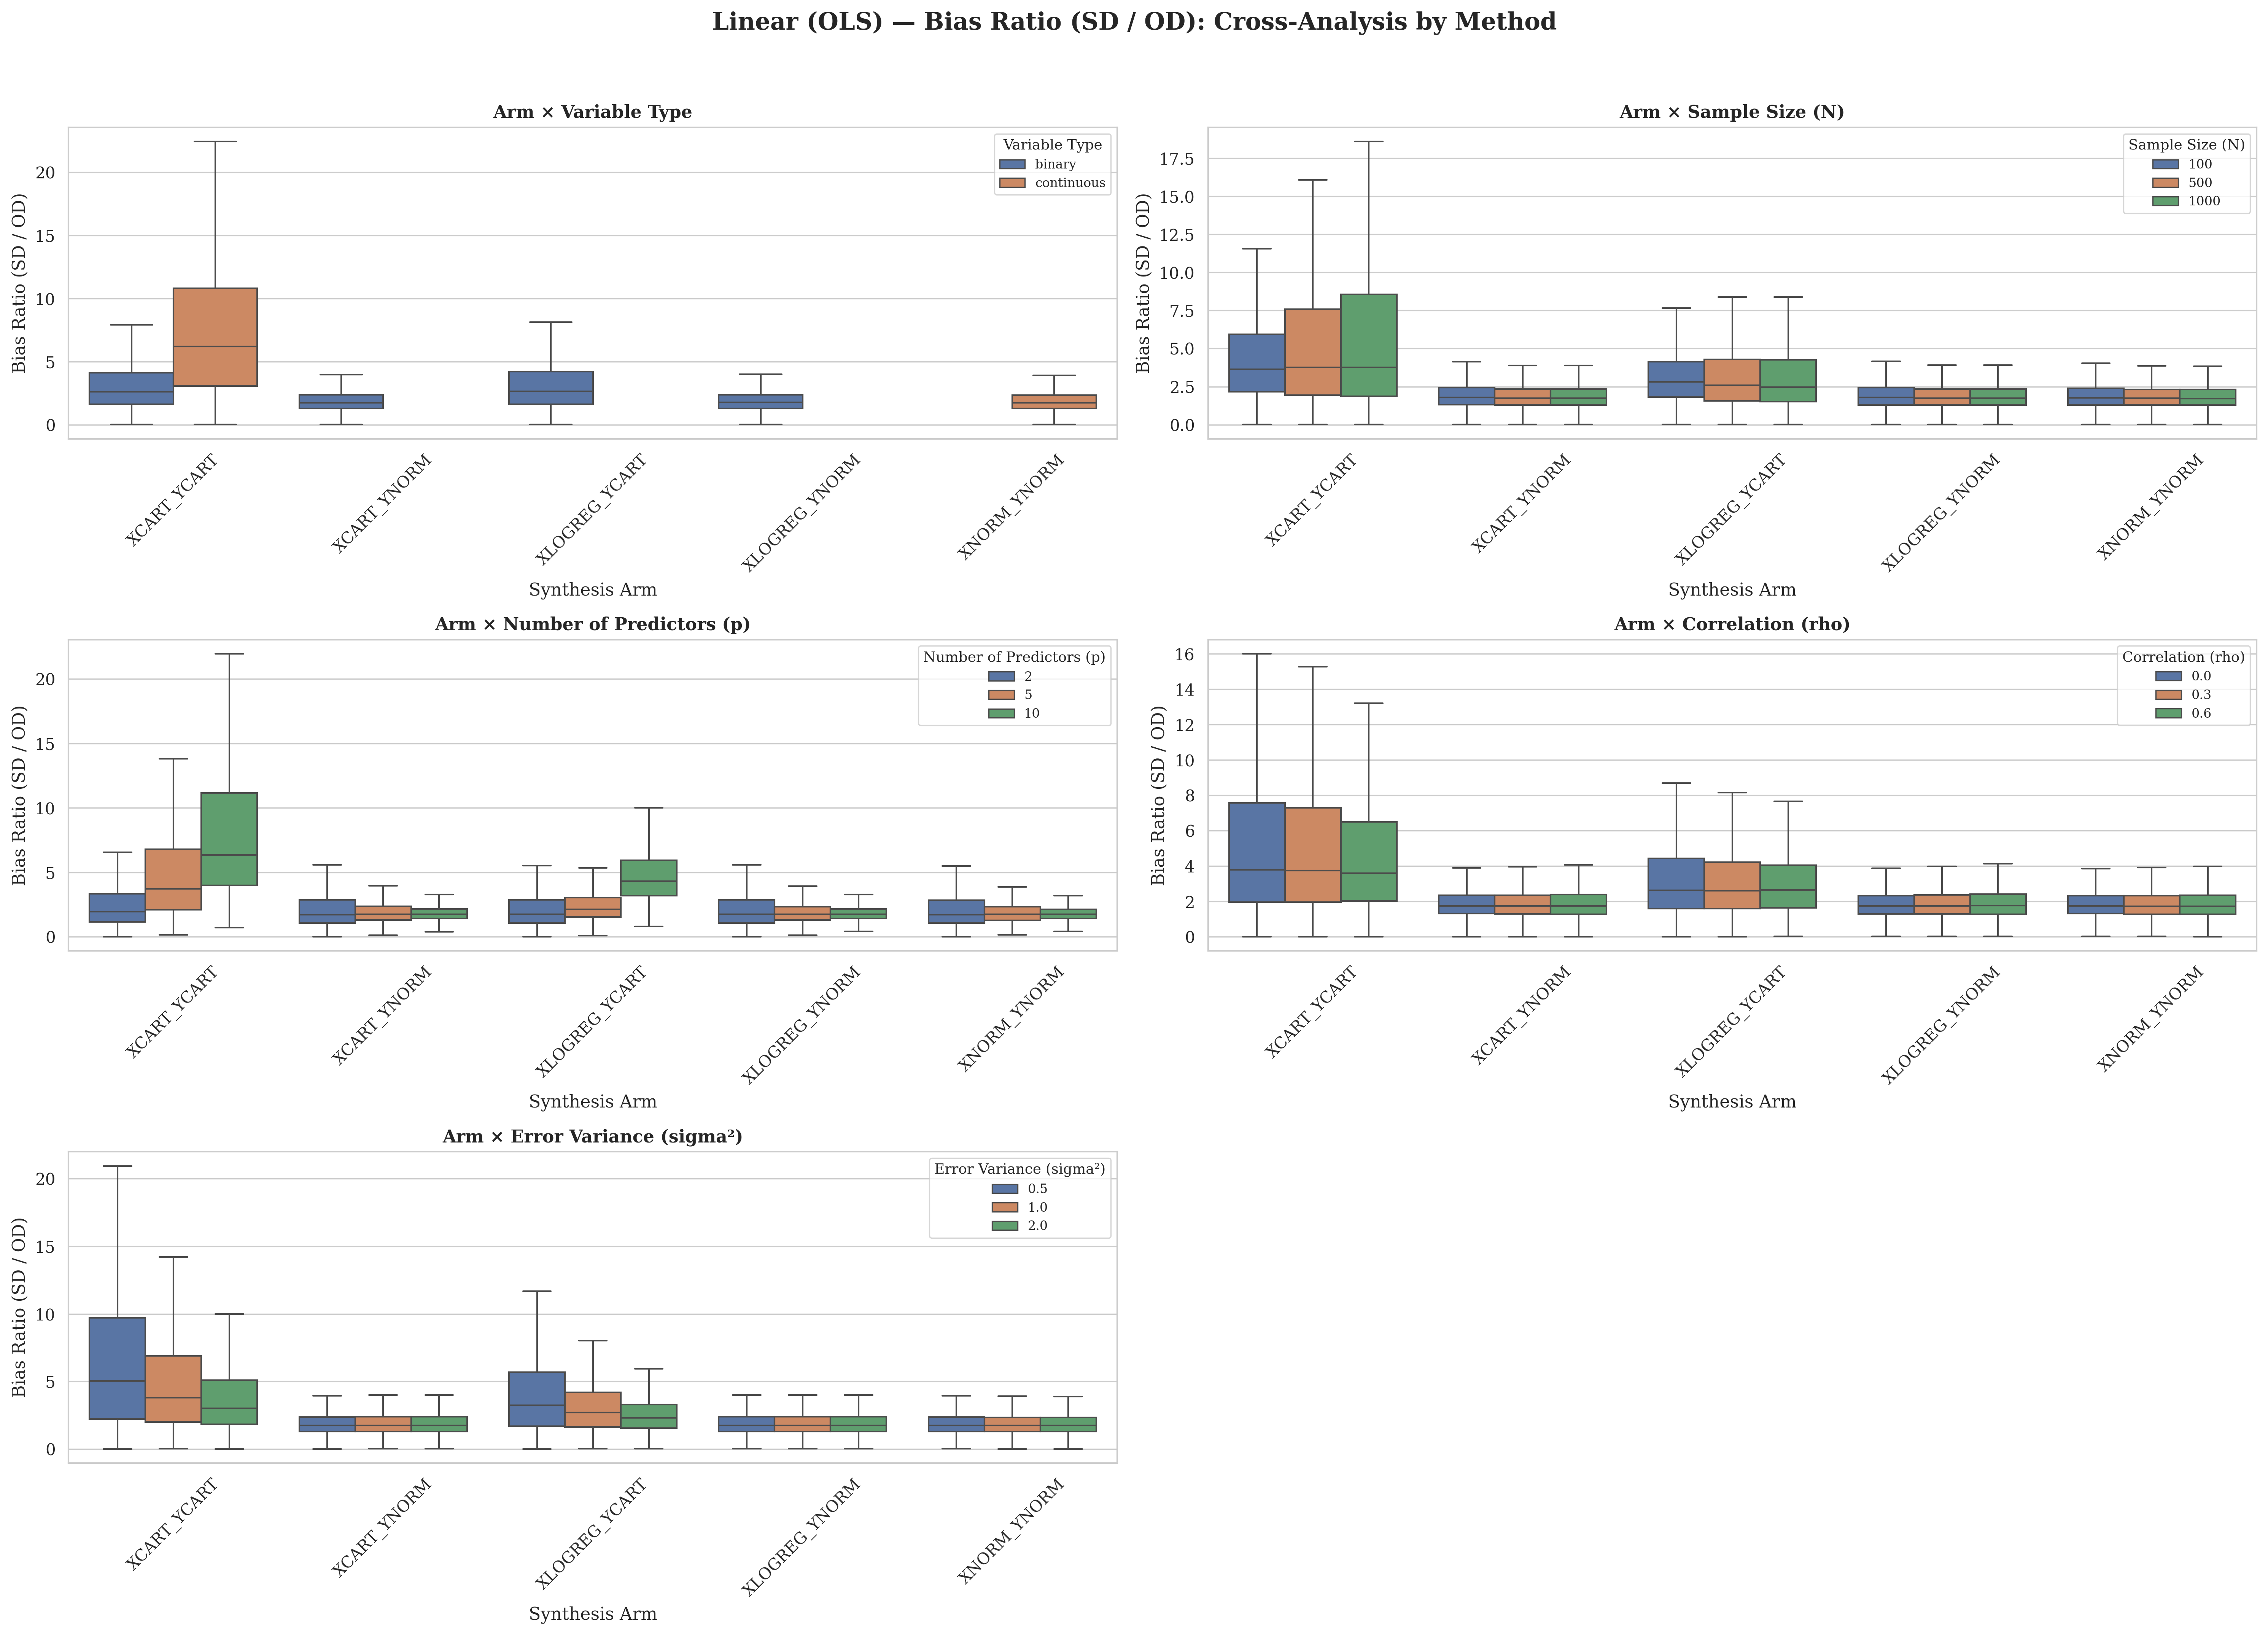
\includegraphics[width=0.7\textwidth]{figures/parts/03_Regression/03_Linear_Results/linear_plot_bias_ratio_by_method.png}
    \caption[Bias Ratio distribution for Linear Regression]{Distribution of the Bias Ratio by synthesis method for Linear Regression.}
    \label{fig:linear-bias-ratio}
    \source{Compiled by the author}
\end{figure}

Figure~\ref{fig:linear-bias-ratio} shows that both methods generally exhibit a low average bias in the linear regression setting. The OLS estimator relies heavily on the covariance structure $\Sigma = \text{Cov}(\mathbf{X})$, which both methods preserve reasonably well in expectation. However, the CART distribution exhibits a wider ``tail'' of high-bias scenarios. One plausible explanation is that tree-based methods partition the continuous space into orthogonal hyper-rectangles; when used to approximate smooth linear gradients, the resulting stepwise structure can introduce noise that shifts some recovered coefficients.

\subsection{Analysis of the Confidence Interval Width Ratio}
Figure~\ref{fig:linear-width-ratio} shows the distribution of the Confidence Interval Width Ratio across synthesis methods for linear regression.

\begin{figure}[H]
    \centering
    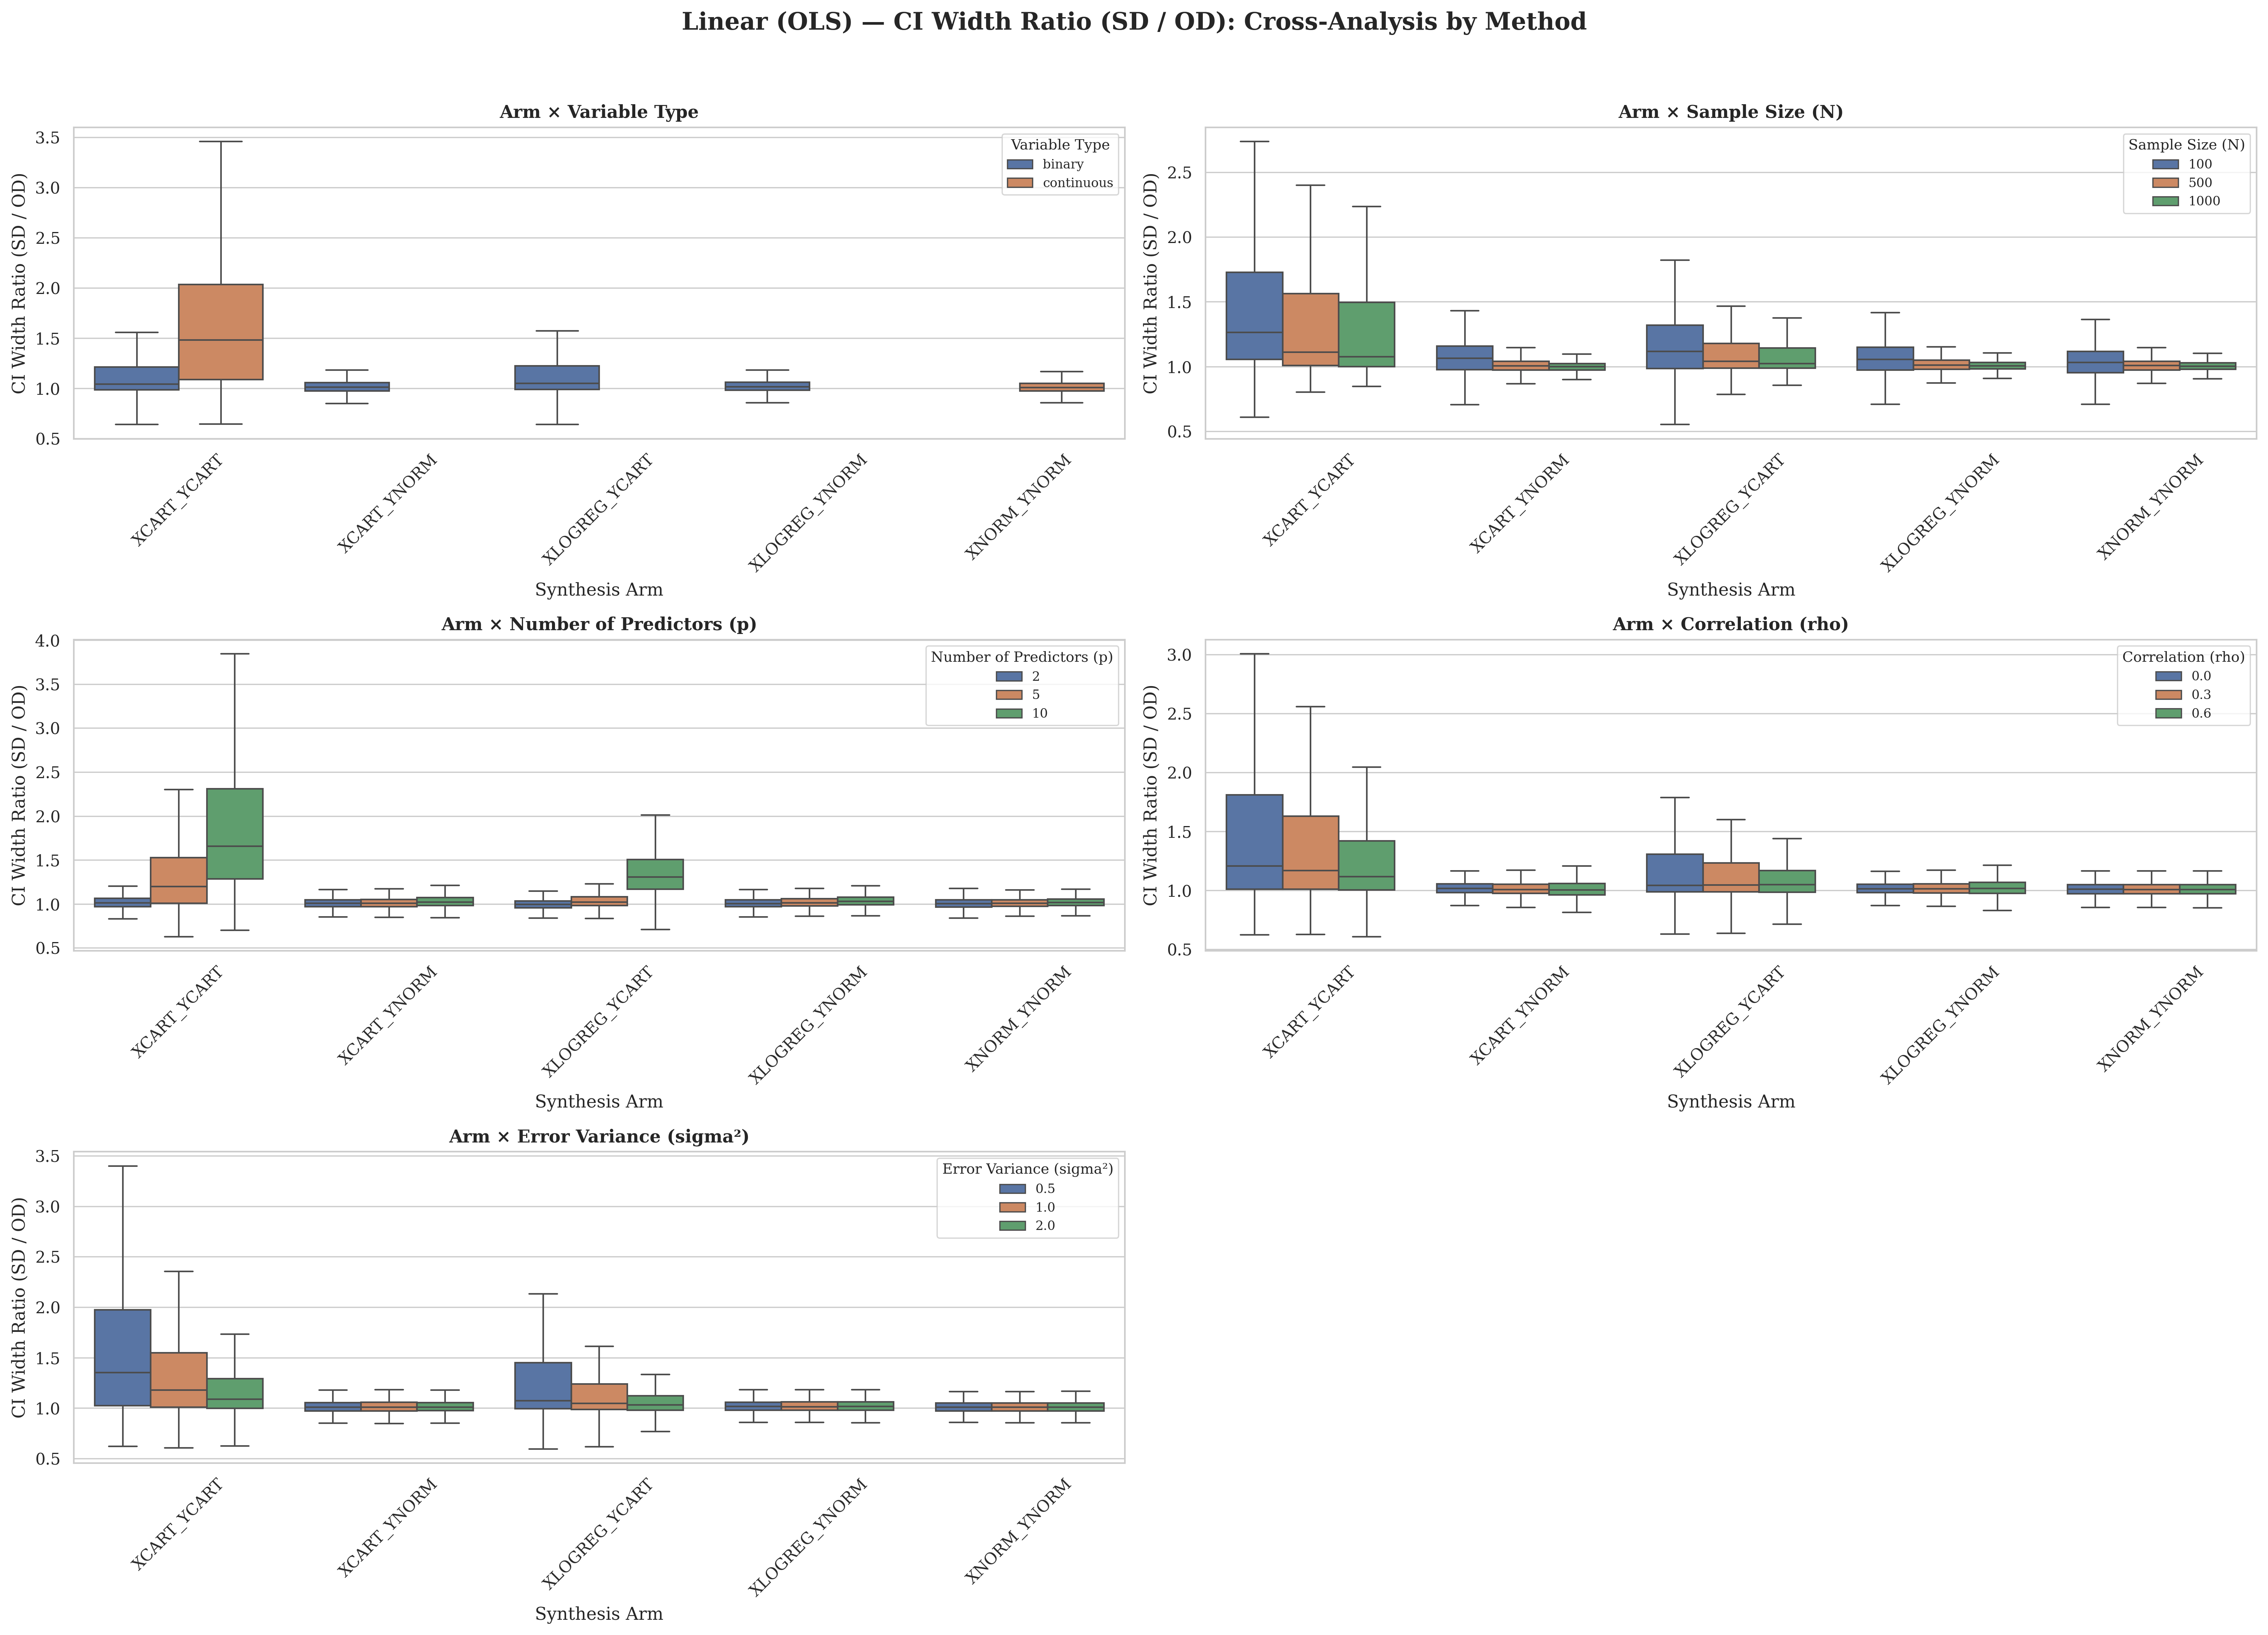
\includegraphics[width=0.7\textwidth]{figures/parts/03_Regression/03_Linear_Results/linear_plot_ci_width_ratio_by_method.png}
    \caption[CI Width Ratio distribution for Linear Regression]{Distribution of the Confidence Interval Width Ratio by synthesis method for Linear Regression.}
    \label{fig:linear-width-ratio}
    \source{Compiled by the author}
\end{figure}

The CI Width Ratio (Figure~\ref{fig:linear-width-ratio}) shows a clear difference in how the two generators manage uncertainty. Parametric methods tend to produce CI widths that are close to those of the original data (Ratio $\approx 1.0$) because they explicitly formulate and inject the Gaussian error term $\epsilon \sim \mathcal{N}(0, \sigma^2)$ during synthesis.

Conversely, CART frequently produces ``overly conservative'' (wider) confidence intervals (Ratio > $1.0$). By modeling local averages within terminal tree nodes, CART introduces additional, unmodeled variance into the synthetic design matrix $\mathbf{X}^{(S)}$. According to the standard error formula $\text{SE}(\hat{\beta}) = \sqrt{\sigma^2 / \sum(x_i - \bar{x})^2}$, an artificially smoothed or disrupted variance profile in the predictors directly inflates the uncertainty bounds of the downstream regression, lowering the overall CIO score despite the relatively low bias.
